We emulated a network following the power law, i.e., $4$ routing 
nodes in the middle to emulate the backbone domains and the rest emulate the access domains in between the backbone nodes and the end hosts. 

Among the $23$ nodes in this topology, we specify $6$ data origins and $6$ data sinks as the end hosts to transfer a batch of data files of different sizes that we randomly acquired from OSG. 
This file batch is transferred between every chosen pair of end hosts. We ran two sets of experiments to collect two sets of raw training data. In the first one, called {\it Partial},
data transfers only happen between the origins and sinks, where every origin node sends all the files in the batch 
to all the receiving nodes in parallel. In the second one, called {\it Complete}, data transfers happen between all the end host pairs. 
The file integrity is being checked at the receiving end host and each file transfer accounts for one data flow and therefore 
a data sample in a training data set. We further parallelized the data transfer process to reduce the emulation time down to about twenty-four hours for this particular network.  

For each experiment, probabilistic integrity error or network impairment via the Chaos Jungle tool is injected to the $54$ link interfaces and $12$ end hosts in sequence with the given probability setting.
For each fault injection scenario, the entire set of {\it Partial} or {\it Complete} data transfers are conducted. Each link interface or node component with fault injected represents a label.  
The receiving node checks if a received file is identical to its original copy via checksum and marks this data transfer as a failure data sample if checksums do not match. 
We treat retransmission as a separate feature for the data samples.  A file could also be missed at the destination due to ultimate transfer failure which is also treated as a failure. 
If the checksum matches, this data transfer becomes a positive data sample in the training data set. Otherwise, it is labeled by the corresponding faulty element.
The final {\it Complete} training data set consists of 8{M} data samples.

Each figure shows five different performance metrics under four scenarios. The five metrics are F1 score with per-flow inference, the accuracy with per-({\it Flow}) inference, and the $Top-1$, $Top-2$, and $Top-3$ accuracy with
the {\it Aggregated Flow} inference. The four scenarios are {\it Partial} and the {\it Complete} data sets with {\it All Features} or only {\it No File features}.

\begin{figure}[!ht]
\begin{center}
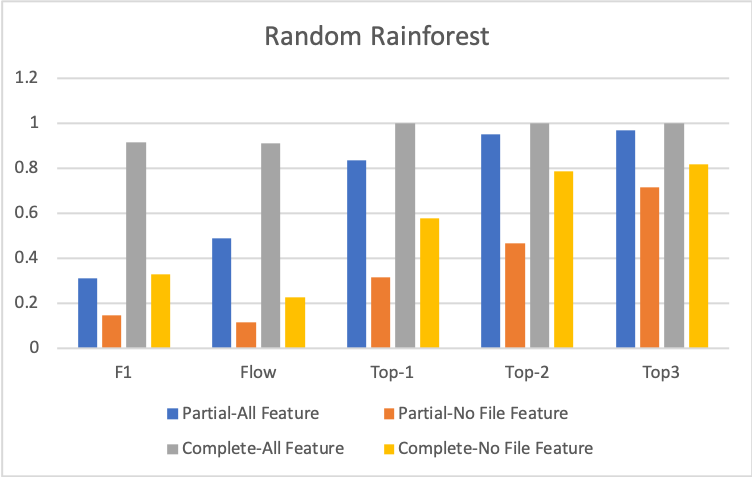
\includegraphics[width=0.4\textwidth]{./figure/rf-accuracy}
\end{center}
\caption{Classification Accuracy with Random Forest Model}
\label{fig:dt}
\end{figure}

Fig.~\ref{fig:dt} presents the results from training random forest models with different data sets. Two prominent observations stand out. 
First, it clearly shows that the model with {\it Complete} data performs significantly better than the {\it Partial} case. This illustrates the importance of sufficient 
coverage of the network path information in the training data set. It also shows that, even without the full coverage of network paths between the network routers, 
the flows between end hosts alone can guarantee very high RCA inference accuracy.   
Secondly, training with {\it All Features} outperforms its {\it No File Features} counterpart by a large margin. This means the file transfer statistics can boost the inference performance.  
We also learned that the file transfer throughput has a bigger impact than the file size, though the result is not shown here. 

When we zoom into more details, we can see that the combined {\it Complete-All Features} data set presents satisfactory performance even with the single flow-based testing data samples with 
both F1 score and accuracy reaching above $0.90$. When the aggregated flow data samples are used for inference, the accuracy scores perfect $1$. The next best scenario is when {\it All Features} presented with 
{\it Partial} data transfer, while the single flow-based inference only achieved under $0.5$ accuracy, the aggregated flow-based inference doubles the accuracy and quickly narrows down the root cause to the 
top $2$ elements. However, without more path coverage, it doesn't achieve perfect accuracy until $Top-10$. For the next two scenarios, the aggregated flow inference helps achieve better performance 
and {\it Complete} path coverage appears more important than the inclusion of file transfer features. However, the best it can achieve is a mere $80\%$ $Top-3$ accuracy.  

In order to gain more insight into the classification accuracy performance, we observed that the majority of mislabeled data in the classification inference are those with labels of end host faults in all the scenarios whose accuracy is less than $1$.  This is because the raw training data set is highly imbalanced due to the different impacts of the injected failures on the data files being transferred (Section~\ref{sub:ml:imbalance}). There are significantly fewer integrity errors caused by the faulty end hosts, \ie, significantly less labeled data in these classes. 

The main techniques to solve the dataset imbalance problem are to rebalance the data via oversampling or downsampling data from different classes. Since the labeled data subsets from the end host failure classes are rather small, the pure downsampling techniques will not improve on the model performance. We focus on two representative oversampling techniques: random and SMOTE as well as two methods that combine oversampling and downsampling in SMOTETomek and SMOTEENN~\cite{imbalance-learn:web}.

For the  {\it Complete-All Features} data set, our analysis indicated that both Random and combined SMOTE methods resulted in similar perfect $Top-k$ performance but slightly reduced flow-based F1 Score and accuracy. SMOTE deteriorated all the metrics. The observations on the  {\it Complete-No File Features} data set are similar. Since the performance of the original model is already perfect for the former case, we only present the results on the two {\it Partial} data sets.

\begin{figure}[!ht]
\begin{center}
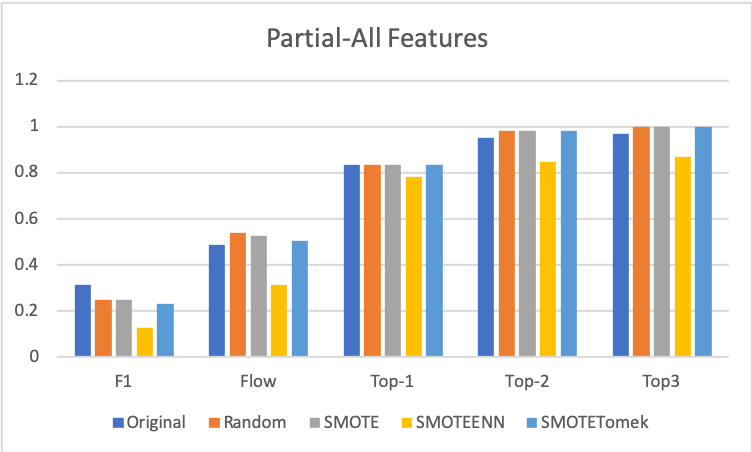
\includegraphics[width=0.4\textwidth]{./figure/partial-all-oversampling}
\end{center}
%\vspace{-0.1in}
\caption{Oversampling with All Features}
\label{fig:os:all}
%\vspace{-0.2in}
\end{figure}

\begin{figure}[!ht]
\begin{center}
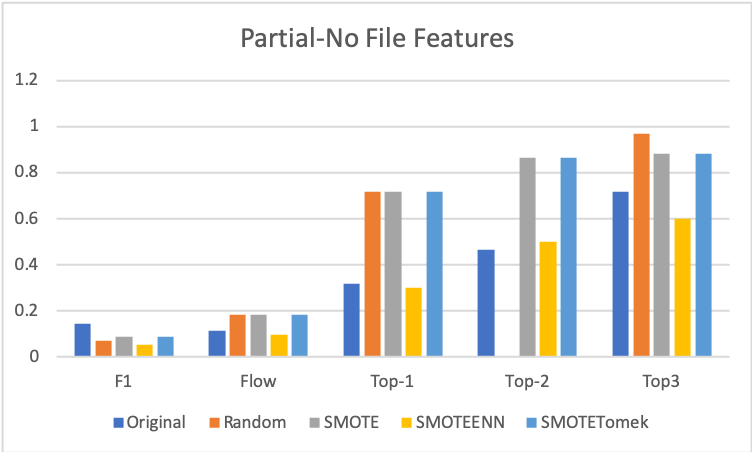
\includegraphics[width=0.4\textwidth]{./figure/partial-nofile-oversampling}
\end{center}
%\vspace{-0.1in}
\caption{Oversampling with No File Features}
\label{fig:os:nofile}
%\vspace{-0.1in}
\end{figure}

The results in Fig.~\ref{fig:os:all} and~\ref{fig:os:nofile} show that the three methods other than the SMOTEENN improve the performance to some extent, especially on the $Top-k$ accuracy measurement. The basic random oversampling demonstrates the best performance improvement in most cases.  The main takeaway is that multiple sampling methods have to be carefully evaluated in order to find the best one.

We also evaluated the multi-granularity classification scheme discussed in Section~\ref{sub:ml:granularity}. For the simulated system, we combine each access router and the end hosts attached to it into one domain and aggregate the related labels into a super label. A random forest model can be trained to achieve $100\%$ accuracy with the basic aggregated flow inference.    
